\begin{figure*}[t]
\centering
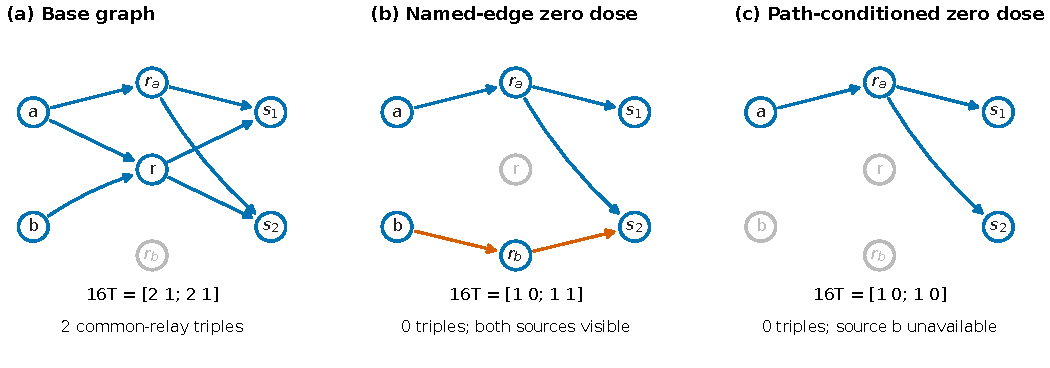
\includegraphics[width=\textwidth]{figures/overview.pdf}
\caption{\textbf{A task-information audit asks a different question from a
motif count.} The same zero common-relay count can hide different source routes.
Only source-to-sink two-hop routes are shown for the reconstructed narrow $k=4$
interventions. Named-edge compensation retains both sources; the path-conditioned
zero dose loses one. Accuracies are archived fits; matrices are post-hoc
reconstructions from release-matched data and archived code.}
\label{fig:overview}
\end{figure*}
